%!TEX encoding = UTF-8 Unicode
%%%%%%%%%%%%%%%%%%%%%%%%%%%%%%%%%%%
%
%  平成29年度 卒業論文 Ver.1.0
%  
%%%%%%%%%%%%%%%%%%%%%%%%%%%%%%%%%%%


%%%%%%%% OPTION %%%%%%%%%
% 想定コンパイラ platex
% 言語 日本語
% 用紙サイズA4
% 文字サイズ12pt
% 段組み 1段組み
% dvi->pdf chainを想定 
% ps->pdf chainならdvipsを指定すること
%%%%%%%%%%%%%%%%%%%%%%%%%
\documentclass[a4paper,12pt,onecolumn,dvipdfmx]{jsarticle}
\usepackage{graphicx}
\usepackage{color}
\usepackage{amsmath}
\usepackage{amsfonts}
\usepackage{amssymb}
\usepackage{listings,jlisting} %コード内に日本語を使う場合はjlisting.styが必要
\usepackage{url}
\usepackage{here}
\usepackage{color}
\newcommand{\diff}[1]{\textcolor{red}{#1}}
\usepackage{longtable}
\usepackage{multirow}
\usepackage{bm}
\usepackage{comment}
\usepackage[subrefformat=parens]{subcaption}
\setlength{\oddsidemargin}{-0.4truemm}   % 25.4 - 0.4 = 25mm
\setlength{\evensidemargin}{-0.4truemm}
\setlength{\textwidth}{160truemm}        % 210 - 25 - 25 = 160mm
\setlength{\topmargin}{-5.4truemm}       % 25.4 - 5.4 = 20mm
\setlength{\headheight}{0mm}
\setlength{\headsep}{0mm}
\setlength{\textheight}{252truemm}       % 297 - 20 - 25 = 252mm
\renewcommand{\baselinestretch}{1.1}
\renewcommand{\thesection}{第\arabic{section}章}

\renewcommand{\lstlistingname}{コード}
\renewcommand{\lstlistlistingname}{コード目次}

%%%%%%%%%%%%%%%%%%%%%%%%%%%%%%%%%%%%%%%%%%%%%%
%
% Fortanのlstset例
%
%%%%%%%%%%%%%%%%%%%%%%%%%%%%%%%%%%%%%%%%%%%%%%
\lstset{language=Python,
	basicstyle=\footnotesize,
	commentstyle=\textit,
	classoffset=1,
	keywordstyle=\bfseries,
	frame=tRBI,framesep=5pt,
	showstringspaces=false,
	numbers=left,stepnumber=1,numberstyle=\footnotesize,
	escapeinside={(@}{@)}
	}
\lstdefinestyle{top}{
	float=t,
	floatplacement=t
	}
\lstdefinestyle{bottom}{
	float=b,
	floatplacement=b
	}


%%%%%%%%% TEXT MAIN %%%%%%%%%

\begin{document}
	\begin{titlepage}
	\vspace*{3zw}
	\Large{東北大学工学部 卒業論文} \par
	\vspace*{5zw}
		\begin{center}
		  \huge{\textbf{\underline{ウェブインタフェースを介した}}} \par
		  \huge{\textbf{\underline{スーパコンピュータ利用環境に関する研究}}} \par
		  \vspace*{10zw}
		  \Large{\underline{機械知能・航空工学科 滝沢研究室}} \par
		  \vspace*{3zw}
		  \Large{\underline{谷澤悠太}} \par
		  \Large{(令和6年3月)} \par
		\end{center}
	\end{titlepage}
	
	\pagenumbering{roman}

	\setcounter{tocdepth}{3}
	\tableofcontents%目次
	\clearpage%ページのつなぎ目
	\listoffigures%図目次
	\listoftables%表目次
	\lstlistoflistings
	\clearpage
	\pagenumbering{arabic}
	%!TEX encoding = UTF-8 Unicode

\section{緒論}
\subsection{背景}
近年,高性能計算 (High Performance Computing,HPC)システムの用途は多様化し,専門知識を持たない利用者が容易にHPCシステムを利用する需要が高まっている.一般的に,コマンド操作に基づいてHPCシステムを操作する利用環境や利用するHPCシステムごとに異なる操作方法により,HPCを専門としない研究者はHPCシステムを使いこなすために多くの学習時間を費やす必要がある.実際にPingらは,学習目的でHPCシステムを初めて利用する学生などはHPCシステム利用環境の構築に多くの時間を費やしてしまい,本来の目的である学問のためのHPCシステムの利用を達成するまでに多大な時間を費やしてしまうという問題を指摘している\cite{cite1}.そこで,従来のコマンド操作に基づく利用環境や,システムごとに異なる利用方法を利用者から隠蔽し,ウェブブラウザを用いて容易かつ統一的にHPCシステムを利用することが可能なウェブインタフェースの研究開発が行われている\cite{OOD_1}.\par
現在用いられているジョブスケジューラには数多くの種類が存在し,今後も多くのジョブスケジューラが開発されることが予想される.そのため,ウェブインタフェースはより多くのジョブスケジューラに対応することが求められる.しかし,既存のウェブインタフェースが新たなジョブスケジューラへの対応をするたびに,開発者はウェブインタフェース本体を改修する必要がある.そのため,ウェブインタフェースの保守性に問題があるといえる.\par

\subsection{目的}
本研究では,スーパーコンピュータ利用環境において,ジョブスケジューラの多様化に伴い発生し得るウェブインタフェースの保守性の問題に着目する.そこで,既存のウェブインタフェースの機能を,ユーザがウェブブラウザ上でHPCシステム利用を可能とする機能 (ウェブ機能)と多様なジョブスケジューラを統一的に取り扱う機能 (スケジューラ抽象化機能)の2つの機能に分離して実装することを考える.既存のウェブインタフェースをウェブ機能とスケジューラ抽象化機能に分離することで,新たなジョブスケジューラに対応させる際のウェブインタフェースの改修箇所はスケジューラ抽象化機能のみとなる.そのため,提案手法を用いて,ウェブインタフェースの保守性の問題を解決することを目的とする.具体的には,既存のウェブインタフェースの機能を分離し,実際のシステムに実装する.実装における動作の確認を行い,提案手法の実現可能性を示す.さらに,提案したウェブインタフェースの機能を定量的に評価することで提案手法の有用性を示す.\par

\subsection{本論文の構成}
本論文は全5章から構成される.第1章では,本研究の背景と目的について述べた.第2章では,関連研究について説明し,既存のウェブインタフェースについて述べる.第3章では,ウェブインタフェースを介したHPCシステム利用環境について説明し,提案手法の実装と動作の確認を行う.第4章では,実装した提案手法の評価結果を示し,その考察を行う.第5章では,本研究の結論と今後の課題を述べる.\par

	%!TEX encoding = UTF-8 Unicode

\section{関連研究}

\subsection{緒言}
本章では関連研究について述べる.はじめに,一般的なHPCシステムの利用方法について説明する.続いて,関連研究であるOpen OnDemandと呼ばれるウェブインタフェースについて説明する.ウェブインタフェースの機能やその設計について説明し,既存のウェブインタフェースの利点を整理する.最後に,既存のウェブインタフェースにおける課題を述べる.

\subsection{HPCシステム利用方法}
HPCシステムとは,コンピュータクラスタの能力を利用して,デスクトップ型コンピュータやノートブック型コンピュータを遥かに凌ぐ速度で計算課題 (ジョブ)を処理し,実行するシステムを指す.このような計算能力の集約によって,様々な科学分野において他の方法では対処できない大きな課題を解決できる.実際に,平均的なデスクトップ型コンピュータは毎秒数十億の浮動小数点演算を実行できる.しかし,HPCシステムは,1秒に数千兆の計算を実行することができることが知られている.例えば,スーパーコンピュータ京は1秒間に約1京回,スーパーコンピュータ富岳は1秒間に約44京回の浮動小数点演算を行うことができる\cite{kei,hugaku}.そのため,大規模な計算に対して,HPCシステムの利用は効果的であるといえる.\par
一般的なHPCシステムの利用の流れを図\ref{fig4}に示す.HPCシステムは数種類のサーバやデータベースから構成される.HPCシステムには,ジョブを実行するために計算を行う計算サーバ (ワーカーノード),ワーカーノードを管理するためのジョブスケジューラが配備されたジョブ管理サーバ (マスターノード),ユーザ情報が保存されたデータベースと連携してログイン情報の管理やユーザリクエストの受け渡しを行うログイン用サーバ,実行するジョブの入出力ファイルなどが保存されたファイル管理用サーバなどが存在する.\par
また,ジョブの実行を依頼するためにはジョブスクリプトファイルを作成する必要がある.ジョブスクリプトファイルとは,ジョブ投入用のシェルスクリプトファイルを指す.ジョブスクリプトファイルは大きく2つの部分で構成され,利用する計算機のリソースや環境を指定する部分と計算機に実行させる処理を記述する部分からなる.コード\ref{job_script}ではSLURMスケジューラのジョブスクリプトの例を示す.1行目はシェバンと呼称され,ファイルに記載されたプログラムが/bin/bashで実行されるということを明示的に記載している.2~6行目では,各ジョブスケジューラごとに定義されている接頭辞 (Slurmの場合は\#SBATCH)を用いて,利用する計算機のリソースや環境を指定する.2行目では,ジョブを投入するキューの名前を指定してる.3行目では,ジョブで使用するプロセス数を指定している.4行目では,実行するジョブの名前を指定している.5行目と6行目では,標準出力ファイルと標準エラー出力ファイルを指定している.なお,\%JはジョブIDに変換される.また,7行目は計算機に実行させる処理を記述する部分であり,プログラム (a.out)を実行する.\par
ユーザは利用したいHPCシステムを遠隔で操作するために自身のコンピュータからユーザ情報を用いて秘密鍵の登録を行った後,ログイン用サーバにSSH接続を用いてログインする.そして,ユーザは利用するジョブスケジューラの種類に応じた形式でジョブスクリプトを作成する.その後,各ジョブスケジューラごとに異なるユーザはジョブの実行を依頼するためのコマンドを用いて,マスターノード上で動作しているジョブスケジューラにジョブの実行を依頼する.ジョブスケジューラはファイル管理用サーバから入力ファイルを受け取り,ワーカーノードはマスターノードの命令に従ってジョブの実行を行う.ジョブ実行時の標準出力,エラー標準出力はファイルに出力され,ジョブ実行後に実行結果を確認することができる.\par

\begin{figure}[tb]
    \centering
    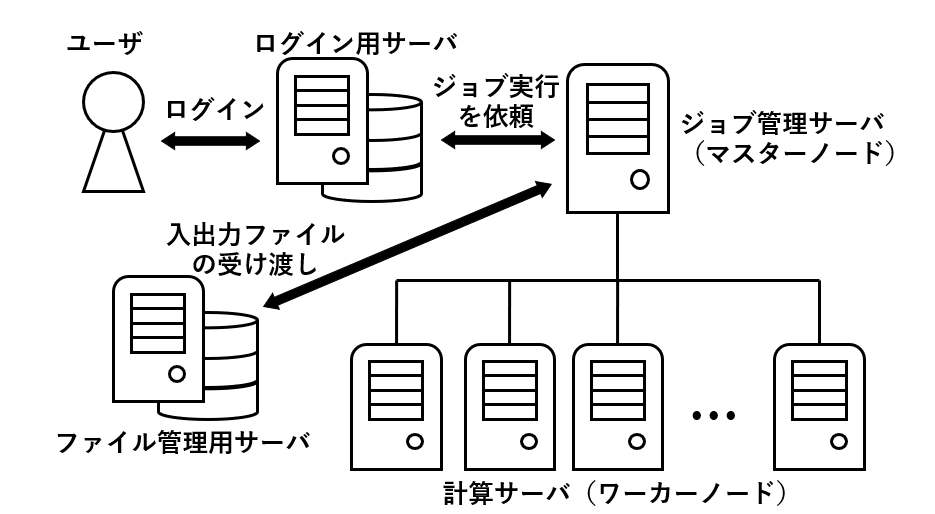
\includegraphics[width=120mm]{./fig/HPCsystem.png}
    \caption{一般的なHPCシステムの模式図}
    \label{fig4}
\end{figure}

\begin{lstlisting}[caption=Slurmのジョブスクリプトファイル作成例, label=job_script]

#!/bin/bash
#SBATCH -p partition1
#SBATCH -n 1
#SBATCH -J example
#SBATCH -o stdout.%J
#SBATCH -o stderr.%J
    
./a.out
    
\end{lstlisting}

\subsection{Open OnDemand}
代表的な関連研究として,Open OnDemand (OOD)とその機能や設計構成を紹介する\cite{cite2,cite3}.OODは米国オハイオ・スーパーコンピューティングセンターが開発したオープンソースソフトウェアであり,ウェブインタフェースを介してHPCシステムを利用できる環境を提供する.ユーザはウェブブラウザ上でHPCシステムを簡単に操作することができ,プラグインやほかのソフトウェアのインストールや設定は不要である.また,リモートデスクトップやJupyter Notebook\cite{jupyternotebook},Visual Studio Codeなどの対話的アプリケーションもウェブブラウザ上から利用することができる.OODは世界的に使われている様々なジョブスケジューラ (PBS Pro\cite{PBS_Pro},Slurm\cite{Slurm},Grid Engine\cite{Grid_Engine},Torque\cite{TORQUE},LSF\cite{LSF}など)に対応しているため,システム間の利用方法の差異を隠蔽している.\par
初めに,OODの機能について説明する.OODは,図\ref{dashboard}に示すダッシュボードと図\ref{homedirectory}に示すユーザのホームディレクトリを管理する画面,図\ref{activejobs}に示すジョブの状態を確認する画面,図\ref{jobcomposer}に示すジョブの管理を行う画面,図\ref{shell}に示すHPCクラスタのシェル操作を行う画面,開発者が任意の追加アプリケーションソフトウェアを導入することができるInteractive Apps画面から構成される.図\ref{homedirectory}に示すホームディレクトリ画面からはユーザのディレクトリを視覚的に操作することができ,ファイルやディレクトリの削除,追加,および編集なども容易に行うことができる.図\ref{activejobs}にはジョブの状態確認を行うActive Jobs画面を示す.ユーザは投入したジョブの状態をリアルタイムで確認することができる.図\ref{jobcomposer}のJob Composerの画面では,ユーザはジョブの作成,投入,削除などをすべてこの画面から行うことができ,HPCシステム内のジョブの管理を行うことができる.図\ref{shell}には,シェル画面を示す.ユーザは連携したHPCクラスタのシェルをウェブブラウザ上から操作することができる.このように,OODは様々な機能やアプリケーションソフトウェアと連携してHPCユーザの利用者支援を行っている.\par
続いて,OODの設計について説明する.OODのクラス図を図\ref{class_diagram}に示す.OODは現在多様なジョブスケジューラに対応しているが,各ジョブスケジューラへの対応はadaptersディレクトリ下に配置される.指定したジョブスケジューラに対応するために,各ジョブスケジューラ用のAdapterスーパークラスのサブクラスが宣言される.サブクラス内部ではジョブの投入を行うsubmitメソッド,クラスターの情報を取得するcluster\_infoメソッド,ユーザ情報を取得するaccountsメソッド,ジョブの情報を取得するinfoメソッド,info\_allメソッド,info\_where\_ownerメソッド,ジョブの状態を取得するstatusメソッド,ジョブの一時停止を行うholdメソッド,ジョブの再開を行うreleaseメソッド,ジョブの削除を行うdeleteメソッドなどが再定義されている.また,各ジョブスケジューラのサブクラス内にはBatchクラスが定義されており,前述したサブクラス内部のメソッドはBatchクラス内部のメソッドを利用して実装されている.例えば,AdapterスーパークラスのサブクラスであるSlurmクラスは,Slurmクラスタにジョブを投入するためのメソッドであるsubmitメソッドを再定義しており,Slurmクラスで定義されたsubmitクラスは内部クラスであるBatchクラスのsubmit\_stringメソッドを用いてジョブの投入を行う.このように,利用するジョブスケジューラのサブクラスで再定義されたメソッドを用いることで,OODは多様なジョブスケジューラに対応することができている.\par
以上のように,OODは視覚的かつ簡単な操作を用いてHPCシステムの利用を行うことができるというメリットを持つ.また,OODは対応しているジョブスケジューラごとにAdapterクラスが宣言されている.そのため,各Adapterクラスを新規作成および改修することで,OODのジョブスケジューラへの対応機能を改修することができる.そのため,多くのコンピューティングセンターで実用化され,OODのユーザ数も年々増加しており,HPC利用環境を提供するウェブインタフェースとして多くの研究開発が行われている.\par

\begin{figure}[t]
    \centering
    \fbox{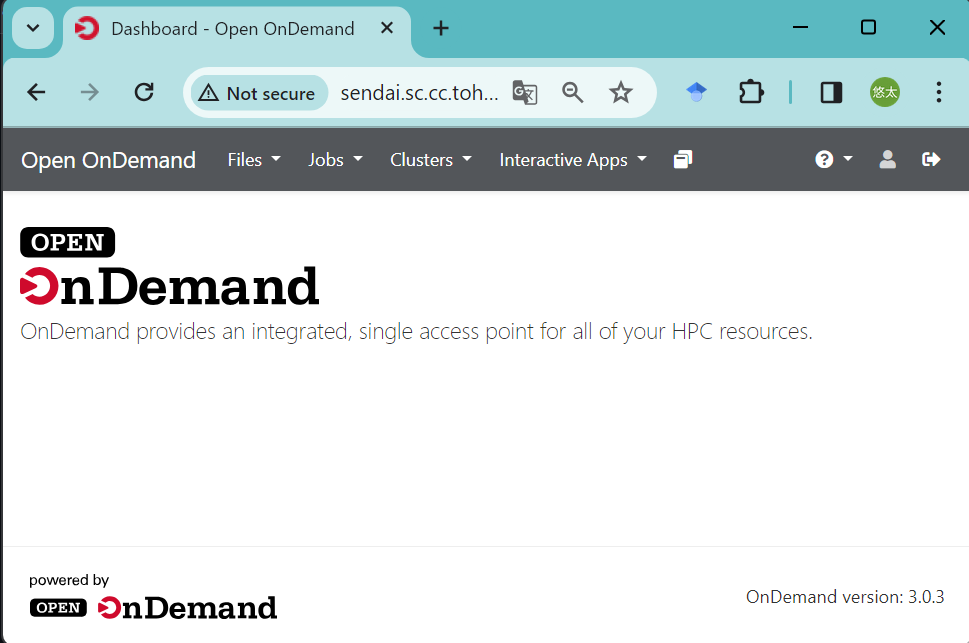
\includegraphics[width=120mm]{./fig/dashboard.png}}
    \caption{ダッシュボード画面}
    \label{dashboard}
\end{figure}

\begin{figure}[t]
    \centering
    \fbox{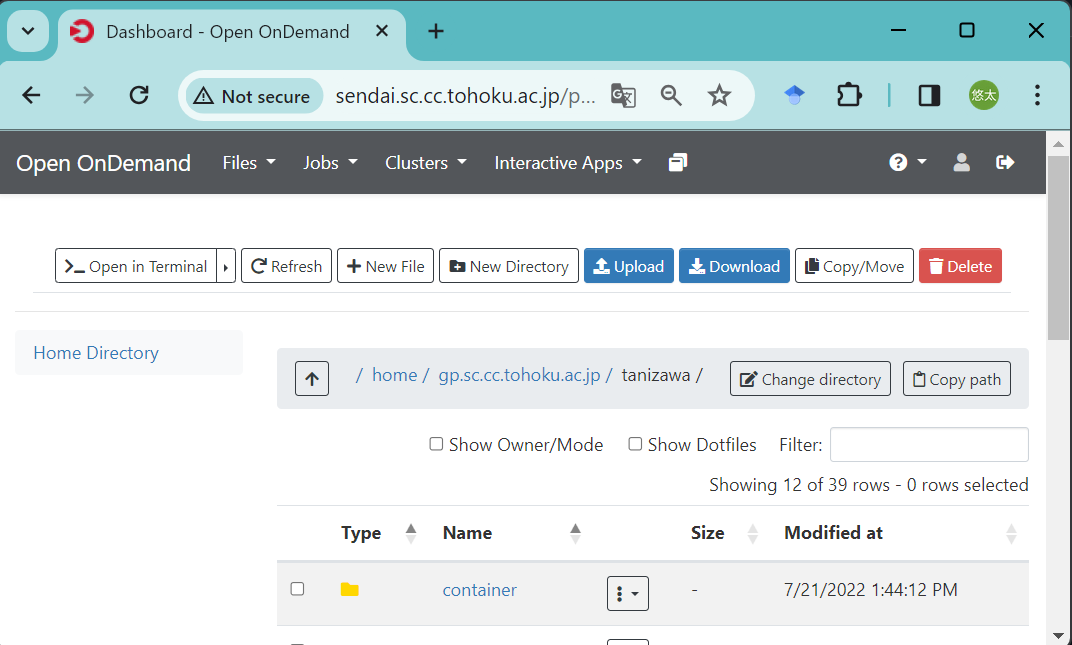
\includegraphics[width=120mm]{./fig/homedirectory.png}}
    \caption{ホームディレクトリ画面}
    \label{homedirectory}
\end{figure}

\begin{figure}[t]
    \centering
    \fbox{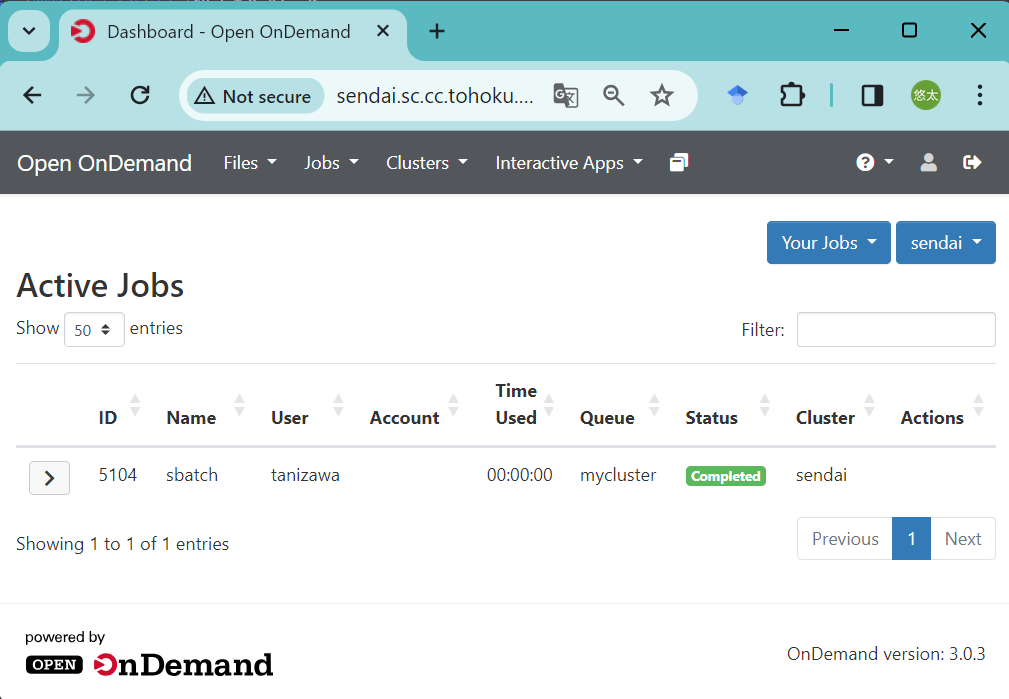
\includegraphics[width=120mm]{./fig/activejobs.png}}
    \caption{Active Jobs画面}
    \label{activejobs}
\end{figure}


\begin{figure}[b]
    \centering
    \fbox{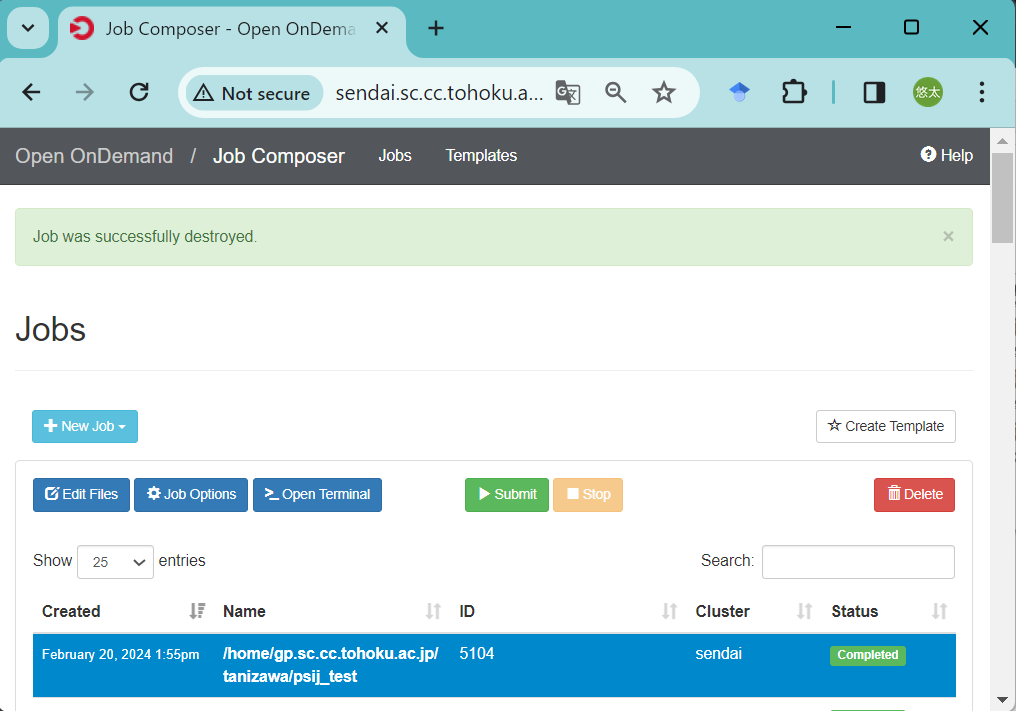
\includegraphics[width=120mm]{./fig/jobcomposer.png}}
    \caption{Job Composer画面}
    \label{jobcomposer}
\end{figure}

\begin{figure}[t]
    \centering
    \fbox{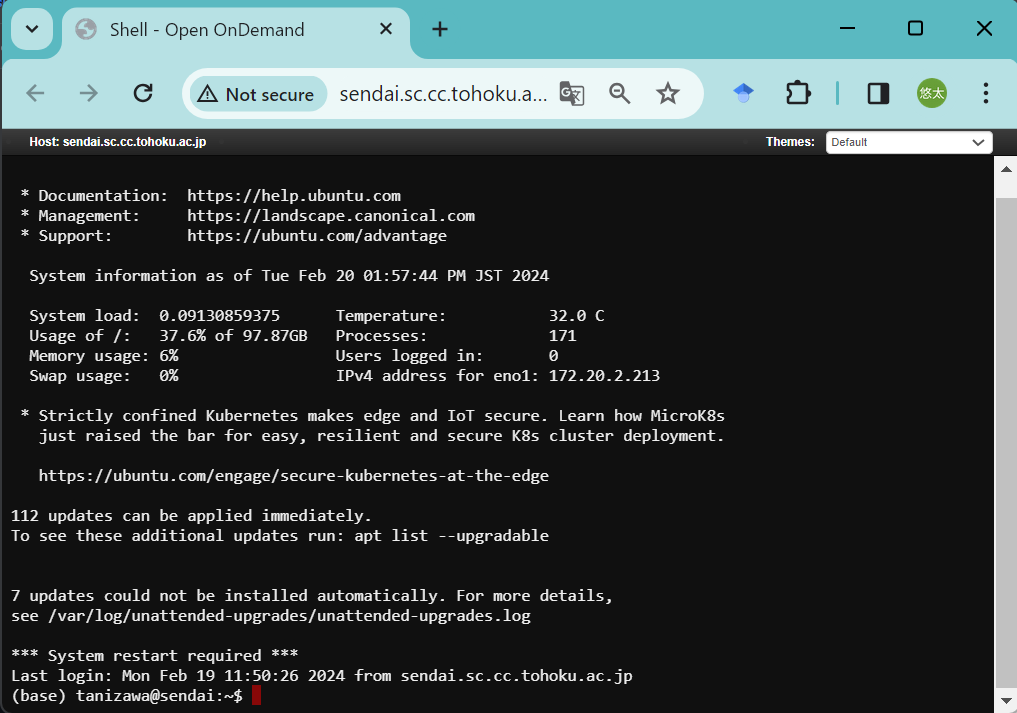
\includegraphics[width=120mm]{./fig/shell.png}}
    \caption{シェル画面}
    \label{shell}
\end{figure}

\begin{figure}[b]
    \centering
    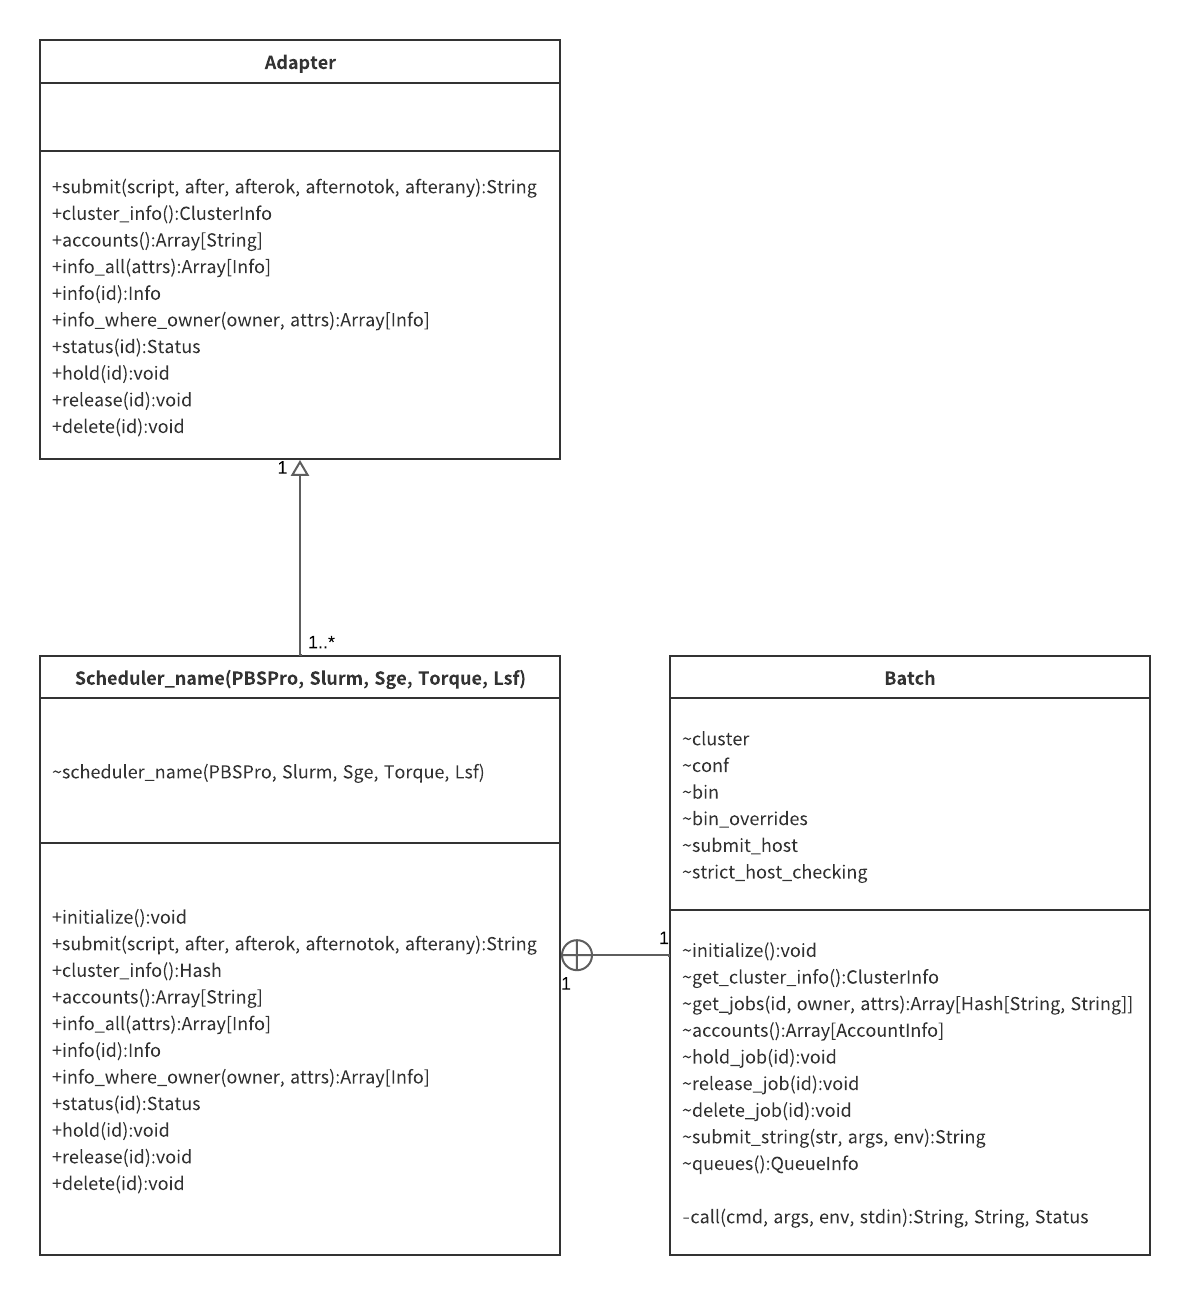
\includegraphics[width=120mm]{./fig/class_diagram.png}
    \caption{OODのクラス図}
    \label{class_diagram}
\end{figure}

\subsection{既存のウェブインタフェースにおける課題}
はじめに,既存のウェブインタフェースであるOODを介したHPCシステム利用環境について説明する.従来手法の模式図を図\ref{fig5}に示す.既存のウェブインタフェースは,各ジョブスケジューラと連携するための機能がウェブインタフェース本体と一体的に実装されている.また,OODはログイン時に認証機構を必要としており,DexとのOpeIDコネクト\cite{dex}\cite{openidconnect}やShibboleth\cite{shibboleth},CAS\cite{CAS}などの認証方法がある.OODは,前述した認証方法に必要な外部の認証用ディレクトリと連携してユーザ情報を管理することで,ウェブブラウザ上での利用空間の提供を行う.また,主要なジョブスケジューラの抽象化を行うことで,統一的な操作環境を提供する.\par

\begin{figure}[b]
    \centering
    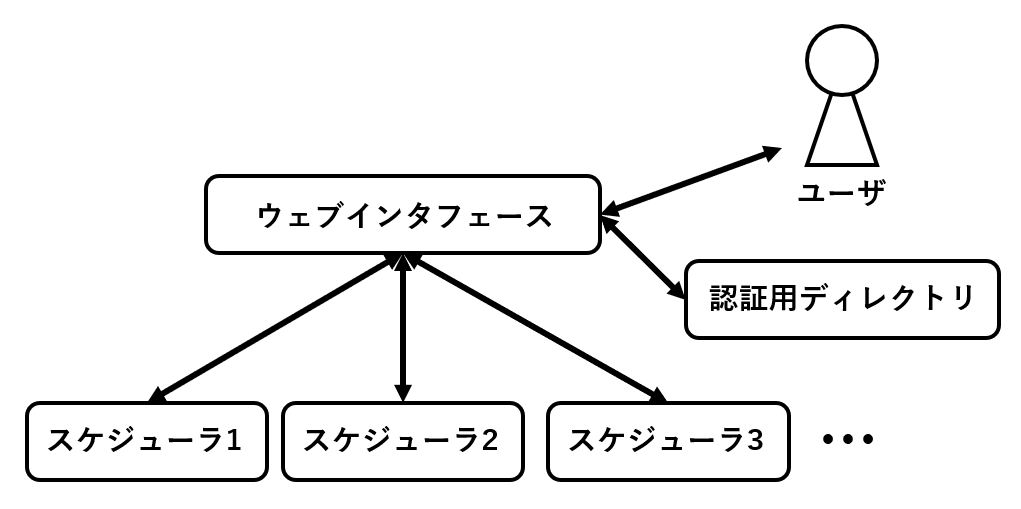
\includegraphics[width=120mm]{./fig/conventional_method.png}
    \caption{従来手法の模式図}
    \label{fig5}
\end{figure}

続いて,既存のウェブインタフェースにおける課題について説明する.OODは視覚的かつ簡単な操作を用いてHPCシステムの利用を行うことができるという利点を持っている.しかし,システム設計上の課題点も考えられる.\par
国内でのウェブインタフェースの実装事例として,スーパコンピュータ富岳でのOODの実装が挙げられる.OODは汎用的なツールであるが,富岳で用いられているジョブスケジューラ (Fujitsu Technical Computing Suite, Fujitsu TCS)に対応していなかったことから,中尾らはOODをFujitsu TCS向けに改修した事例を報告している\cite{cite4}.改修ではAdapterスーパークラスで定義されている下記のメソッドをFujitsu TCS用に実装している.\par

\textbf{submit} ジョブの投入\par
\textbf{delete} ジョブの削除\par
\textbf{status} ジョブの状態を取得\par
\textbf{hold} ジョブの一旦停止\par
\textbf{release} ジョブの再開\par
\textbf{info} ジョブの情報を取得\par
\textbf{info\_all} 全ジョブの情報を取得\par
\textbf{cluster\_info} HPCシステムの情報を取得\par
\textbf{supports\_job\_arrays} バルクジョブのサポートの可否\par
\textbf{directive\_prefix} ジョブスケジューラで用いられる接頭辞の取得 (Fujitsu TCSの場合はPJM)\par

さらに,本来OODに対応しているジョブスケジューラでは図\ref{activejobs}に示すActive Jobs画面のID番号の左にあるボタンをクリックすると,ジョブの詳細情報が表示される.しかし,Fujitsu TCSのようなOODに未対応であるジョブスケジューラは,ジョブの詳細が表示されない.そこで中尾らはFujitsu TCS用に詳細情報が表示されるようにActive Jobs画面の改修を行ったことも報告している\cite{cite4}.\par
ほかにも様々なジョブスケジューラが存在し,今後も登場することを考えると,ジョブスケジューラがの種類が増えるごとにOOD本体を直接改修する方法では保守性に問題があるといえる.\par


\subsection{結言}
本章では,関連研究について述べた.はじめに一般的なHPCシステムの利用方法について説明した.HPCシステムの利用方法について説明し,基礎的な知識を解説した.その後,Open OnDemandと呼ばれるウェブインタフェースについてその機能と設計について説明した.OODを用いることによる影響は大きく,HPCシステムのユーザに多くの利点をもたらすことができると考えられる.また,内部の設計を理解することで,OODのジョブスケジューラへの対応機能の改修方法を理解することができた.最後に,既存のウェブインタフェースについて,国内でのOODの実装例を参考にして課題点を述べた.ユーザに快適なHPC利用空間を提供するという利点に反して,システムの保守性が課題点として挙げられる.次章では,本章で述べた既存のウェブインタフェースにおける課題である保守性を考慮した手法を提案し,その実装を行う.\par
	%!TEX encoding = UTF-8 Unicode

\section{内容2}
統計学において,残差平方和 $E = \sum_{n=1}^N (y_n-(ax_n+b))^2$ は残差の平方の和である.

\subsection{内容2-1}

統計学において,残差平方和は残差の平方の和であり,以下の式で表される.

\begin{equation}
    E = \sum_{n=1}^N (y_n-(ax_n+b))^2
\end{equation}


	%!TEX encoding = UTF-8 Unicode
\section{実装評価}
\subsection{緒言}
本章では,前章で実装した提案手法を用いて,実装評価を行った結果について説明する.はじめに,提案手法の評価を行った際の評価環境と評価条件について説明する.その後,提案手法の実装において考慮すべき実行時のオーバヘッドの測定結果について,表と図を用いて定量的に説明する.\par

\subsection{評価環境}
はじめに,評価環境について説明する.ウェブインタフェースをウェブ機能とスケジューラ抽象化機能に分けたことによって両者の連携時のオーバヘッドの発生が懸念されるため,その影響を定量的に評価する.本実装においては,OODがシェルを介してPSI/JのPythonスクリプトを実行するため,そのオーバヘッドによる影響を評価する.\par
評価には,Selenium\cite{cite6}と呼ばれるウェブページの自動制御ライブラリを用いる.機能の分離前と分離後を比較したいため,OODがNQSVに対応していないことから評価環境として疑似AOBAクラスタを用いることはできない.そこで,実験用に用意したSlurmのHPCクラスタを用いて機能分離に伴うオーバヘッドの評価を行う.ローカルホストからOODホストサーバのウェブポータルにアクセスして,ユーザ名とパスワードを用いてログインする.ダッシュボード画面からJob Composer画面に移動し,NewJobボタンを押下する.選択肢の中からFrom Specified Passを選択してジョブが配置されたディレクトリ,ジョブスクリプトのファイル名,実行するクラスタ名を選択して,ジョブの作成と投入を行う.投入したジョブの状態はsqueueコマンドにより確認し,コマンドの出力結果によってジョブの実行完了を確認する.NewJobボタンを押下した時刻から,そのジョブの実行を完了した時刻までを計測し,ジョブのターンアラウンドタイムとする.\par

\subsection{評価条件}
評価条件について説明する.ジョブの投入を1~10回連続で行い,そのターンアラウンドタイムを計測してPSI/Jを経由する場合と経由しない場合を比較する.ターンアラウンドタイムは1~10回の連続投入でそれぞれ20回ずつ計測し,その平均値をとることで誤差を考慮した結果を得る.また,ジョブを1~100回連続投入した際のターンアラウンドタイムの比較も行った.ジョブの連続投入数は1回から開始して10回ずつ増やしていき,ジョブ数を大きくした場合の結果を得る.\par

\subsection{実行時オーバヘッドの評価}
実行時のオーバヘッドの評価を行う.1~10回のジョブの連続投入により得られた評価結果の実データを表\ref{PSIJ}と表\ref{SLURM}に示す.ジョブを1回投入した場合のターンアラウンドタイムはどちらの場合も30秒弱であるがPSI/Jを経由しない場合の方が若干早いことがわかる.また,ジョブを10回連続投入すると,ターンアラウンドタイムは150秒弱であり,かなりの時間を要することがわかる.この場合も,PSI/Jを経由しない場合の方がターンアラウンドタイムは数秒短いことがわかる.続いてこの実データをグラフとして図\ref{fig8}および図\ref{fig9}に可視化する.図\ref{fig8}では機能分離前後でのターンアラウンドタイムの比較を示す.横軸は連続して投入したジョブの数,縦軸はターンアラウンドタイムを示す.図\ref{fig9}はジョブ実行時のオーバヘッドを示す.横軸は連続して投入したジョブの数,縦軸はジョブ実行時のオーバヘッドを示す.図\ref{fig8}からPSI/Jを経由した提案手法の方がわずかにターンアラウンドタイムが大きいことがわかり,どちらの場合も連続投入したジョブの数に線形比例して増加していることがわかる.また図\ref{fig9}から,ジョブの連続投入回数が多くなればなるほど両者の実行時オーバヘッドの差が大きくなっていることがわかる.\par

\begin{table}[tb]
    \centering
    \caption{PSI/Jを経由した場合の評価結果}
    \begin{tabular}{|c|c|}
    \hline
    ジョブ連続投入数 & ターンアラウンドタイム{[}s{]} \\ \hline
    1        & 24.0               \\ \hline
    2        & 28.6               \\ \hline
    3        & 51.6               \\ \hline
    4        & 64.8               \\ \hline
    5        & 78.1               \\ \hline
    6        & 91.0               \\ \hline
    7        & 105.6              \\ \hline
    8        & 118.3              \\ \hline
    9        & 131.9              \\ \hline
    10       & 146.5              \\ \hline
    \end{tabular}
    \label{PSIJ}
\end{table}

\begin{table}[tb]
    \centering
    \caption{PSI/Jを経由しない場合の評価結果}
    \begin{tabular}{|c|c|}
    \hline
    ジョブ連続投入数 & ターンアラウンドタイム{[}s{]} \\ \hline
    1        & 23.0               \\ \hline
    2        & 37.6               \\ \hline
    3        & 49.7               \\ \hline
    4        & 62.5               \\ \hline
    5        & 75.4               \\ \hline
    6        & 87.9               \\ \hline
    7        & 101.5              \\ \hline
    8        & 114.6              \\ \hline
    9        & 127.3              \\ \hline
    10       & 139.9              \\ \hline
    \end{tabular}
    \label{SLURM}
\end{table}

\begin{figure}[tb]
    \centering
    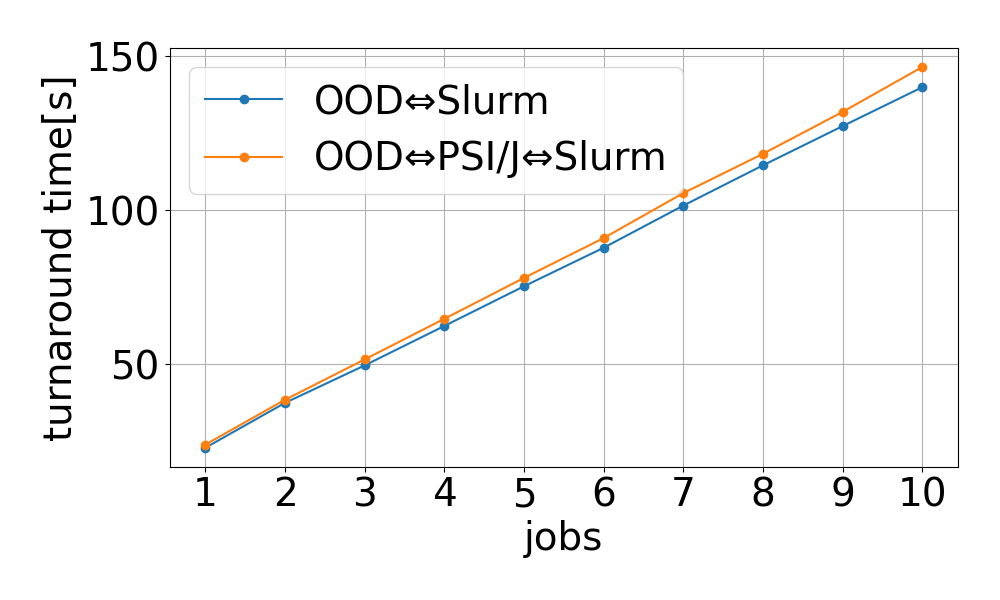
\includegraphics[width=120mm]{./fig/ave_1-20.png}
    \caption{機能分離前後でのターンアラウンドタイムの比較}
    \label{fig8}
\end{figure}
  
\begin{figure}[tb]
    \centering
    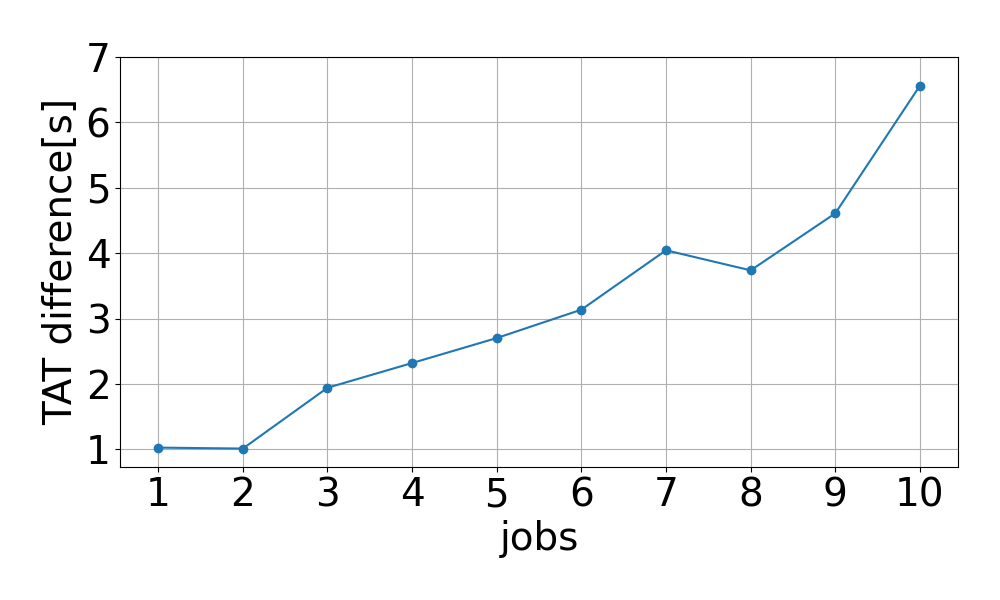
\includegraphics[width=120mm]{./fig/ave_diff_1-20.png}
    \caption{実行時オーバーヘッドの差}
    \label{fig9}
\end{figure}


ジョブを1~100回連続投入した際の機能分離前と機能分離後のターンアラウンドタイムの評価結果を図\ref{fig10}に示す.横軸は連続して投入したジョブの数,縦軸はターンアラウンドタイムを示す.1~10回の連続投入の場合と同じく,PSI/Jを経由した場合の方がわずかにターンアラウンドタイムが大きくなっており,連続投入するジョブ数を大きくしても極端にオーバヘッドに差が出ることはないということがわかった.\par
様々なジョブの連続投入回数でのターンアラウンドタイムの結果から,ジョブ実行時のオーバヘッドを測定した.その結果から,ジョブの連続投入回数に依らず,PSI/Jを経由した場合のオーバヘッドは,PSI/Jを経由しない場合のターンアラウンドタイムの5%以内に収まり,提案手法によって生じるオーバヘッドは十分無視できるといえる.\par

\begin{figure}[tb]
    \centering
    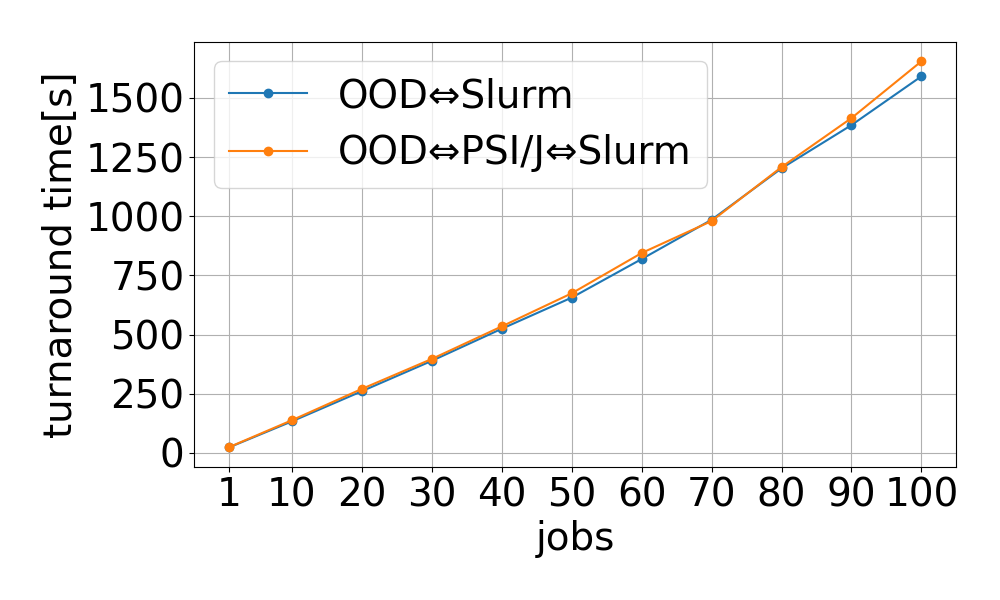
\includegraphics[width=120mm]{./fig/100jobs.png}
    \caption{ジョブ数を増加した際のターンアラウンドタイムの比較}
    \label{fig10}
\end{figure}

\subsection{結言}
本章では,実際にジョブの投入を行った際の提案手法の実装の評価結果を示した.はじめに,評価を行う環境について説明した.その後,機能の分離前後で生じるオーバヘッドを測定する際の評価条件について説明した.これらの評価環境と評価条件により得られた評価結果により,提案手法により生じるオーバヘッドは充分小さいため実用上は問題ないということを示した.\par
	%!TEX encoding = UTF-8 Unicode
\section{結論}





	\addcontentsline{toc}{section}{\bibname}
	\bibliographystyle{junsrt}
	\bibliography{bibpaper}
	%!TEX encoding = UTF-8 Unicode
\section*{謝辞}
本研究を進めるにあたり,滝沢寛之教授には,研究方針から論文の執筆まで様々な点でご支援いただきました.心より感謝申し上げます.また,下村陽一特任准教授と高橋慧智助教授にも,研究活動に関する様々な助言を頂きました.心より感謝申し上げます.また,本研究室所属の先輩方に於かれましても,日頃のゼミ等で研究に対する助言を頂きました.心より感謝申し上げます.最後に日頃から支えて頂いていた家族や友人に感謝申し上げます.\par
\rightline{令和6年3月4日谷澤悠太}

\end{document}
